
\begin{center}
    \textbf{Задача 3.1 --- 9}
\end{center}

\underline{\textbf{Условие:}}

По контуру в виде квадрата со стороной $ a = 20 $ см идет ток $ I = 50 $ A. Определить магнитную индукцию $ B $ в точке пересечения диагоналей квадрата.

\underline{\textbf{Решение:}}

Изобразим схему контура:

\begin{figure}[hpt!]
    \centering
    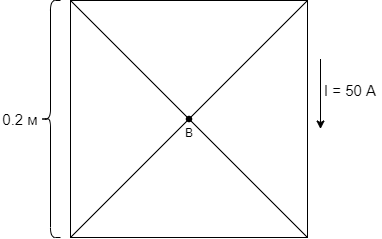
\includegraphics[width=0.8\linewidth]{photo/3-1-9}
\end{figure}

$ B = \sum{B_i} = B_1 + B_2 + B_3 + B_4 $\\

$ 
B_1 = 
\dfrac
{\mu \mu_0 I}
{4 \pi r} 
(\cos{\alpha_1} - \cos{\alpha_2}) 
$\\

$ \alpha_1 = 45^o $, 
$ \alpha_2 = 135^o $ => 

$ \cos{\alpha_1} = \dfrac{\sqrt{2}}{2} $,
$ \cos{\alpha_2} = -\dfrac{\sqrt{2}}{2} $

$ B_1 = B_2 = B_3 = B_4 $ => $ B = 4B_1 $

$ r = \dfrac{a}{2} $, 
$ \mu = 1 $, 
$ \mu_0 = 4\pi * 10^{-7} $, 

$ B = 
\dfrac{4\mu_0I\sqrt{2}}{4\pi 0,1} = 
\dfrac{4\pi 4 \sqrt{2} * 50 * 10^{-7}}{4\pi 0,1} =
200 \sqrt{2} * 10^{-8} = 
284 $ мкТл
\\

\underline{\textbf{Ответ:}}
$ 284 $ мкТл
